\documentclass[border=3mm]{standalone}
\usepackage{tikz}
\usetikzlibrary{arrows, shapes.gates.logic.US, shapes.gates.logic.IEC, calc}

\tikzset{
    my-nand-gate/.style={
        nand gate US, draw, rotate=0, logic gate inputs=nn
    },
    my-nand3-gate/.style={
        nand gate US, draw, rotate=0, logic gate inputs=nnn
    },
    my-not-gate/.style={
      not gate US, draw, logic gate inputs=nn
    },
    my-branch/.style={
        fill, shape=circle, minimum size=3pt, inner sep=0pt
    },
}

\begin{document}

\resizebox{20cm}{!}{

    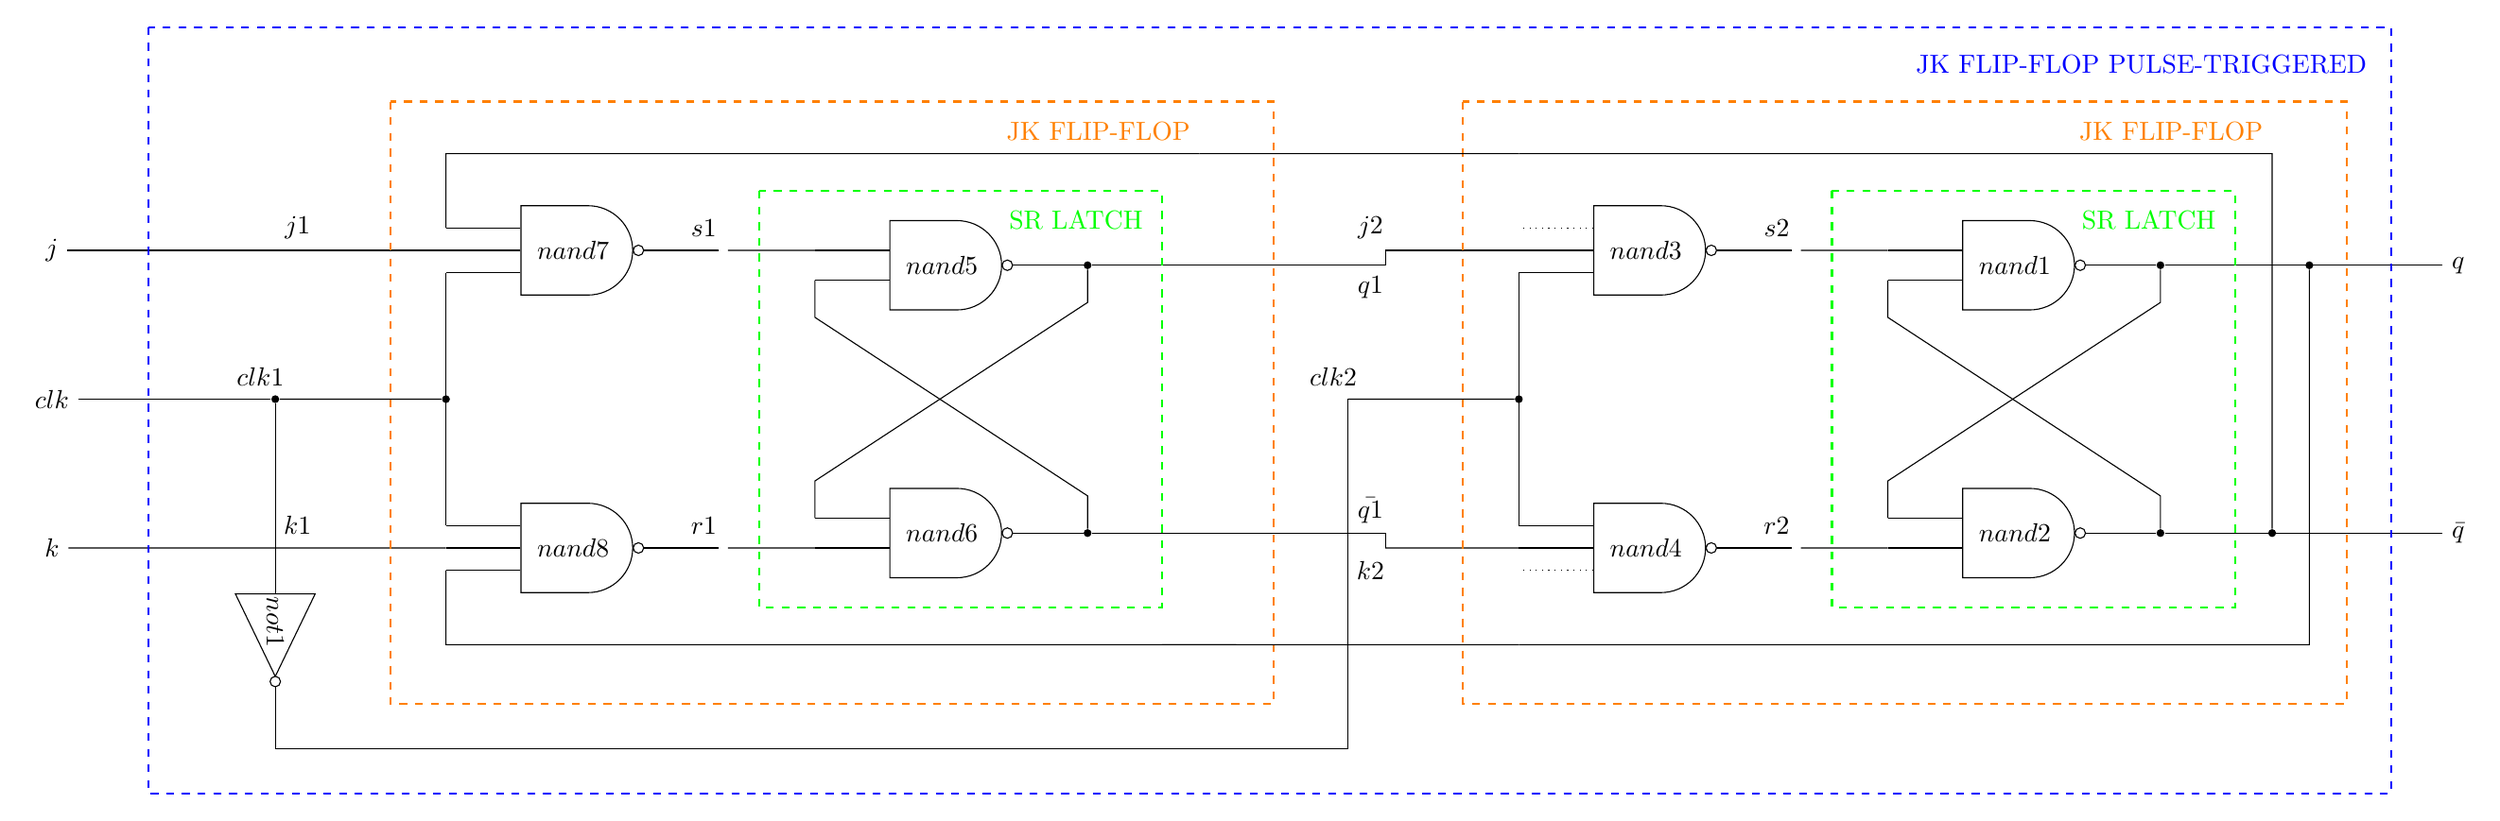
\begin{tikzpicture}[label distance=2mm]

        % JK FLIP-FLOP PULSE TRIGGERED ----------------------------------------------------------------

        % INPUTS - JK FLIP-FLOP
        \node[] (J)   at (0, 0)            {\normalsize $j$};
        \node[] (CLK) at ($(J) + (0, -2)$) {\normalsize $clk$};
        \node[] (K)   at ($(J) + (0, -4)$) {\normalsize $k$};

        % ---------------------------------------------------------------------------------------------
        % JK FLIP-FLOP - MASTER -----------------------------------------------------------------------
        % ---------------------------------------------------------------------------------------------
        % POSITION, COORDINATE, CHANGE CLK NAME AND ADJUST SPACING IF NEEDED

        % INPUTS - JK FLIP-FLOP
        \node[]          (J1)   at ($(J)  + (3.5, 0)$)  {}; *****POSITION, NAME CHANGE*****
        \node[my-branch] (CLK1) at ($(J1) + (-.5, -2)$) {}; *****POSITION, COORDINATE AND CHANGE NAME*****
        \node[]          (K1)   at ($(J1) + (0, -4)$)   {}; *****POSITION, NAME CHANGE*****

        % LABEL IT
        \node at ($(J1)   + (-.2, .3)$) {\normalsize $j1$};
        \node at ($(CLK1) + (-.2, .3)$) {\normalsize $clk1$};
        \node at ($(K1)   + (-.2, .3)$) {\normalsize $k1$};

        % NAND7, WIRES AND CONNECTOR POINTS
        \node[my-nand3-gate](NAND7)    at ($(J1) + (3.5, 0)$)            {\normalsize $nand7$};
        \coordinate[]       (NAND7IN1) at ($(NAND7.input 1) + (-1, 0)$) {};
        \coordinate[]       (NAND7IN2) at ($(NAND7.input 2) + (-1, 0)$) {};
        \coordinate[]       (NAND7IN3) at ($(NAND7.input 3) + (-1, 0)$) {};
        \coordinate[]       (NAND7OUT) at ($(NAND7.output)  + (1, 0)$)  {};
        \draw (NAND7.input 1) -- (NAND7IN1);
        \draw (NAND7.input 2) -- (NAND7IN2);
        \draw (NAND7.input 3) -- (NAND7IN3);
        \draw (NAND7.output)  -- (NAND7OUT);
        
        % NAND8, WIRES AND CONNECTOR POINTS
        \node[my-nand3-gate](NAND8)    at ($(K1) + (3.5, 0)$)            {\normalsize $nand8$};
        \coordinate[]       (NAND8IN1) at ($(NAND8.input 1) + (-1, 0)$) {};
        \coordinate[]       (NAND8IN2) at ($(NAND8.input 2) + (-1, 0)$) {};
        \coordinate[]       (NAND8IN3) at ($(NAND8.input 3) + (-1, 0)$) {};
        \coordinate[]       (NAND8OUT) at ($(NAND8.output)  + (1, 0)$)  {};
        \draw (NAND8.input 1) -- (NAND8IN1);
        \draw (NAND8.input 2) -- (NAND8IN2);
        \draw (NAND8.input 3) -- (NAND8IN3);
        \draw (NAND8.output)  -- (NAND8OUT);

        % INPUT CONNECTIONS
        \draw (J) -- (NAND7IN2);
        \draw (K) -- (NAND8IN2);

        % INTERNAL WIRES - CLOCK
        \draw (NAND7IN3) -- (NAND8IN1) node[my-branch, pos=1/2] (CLKBRANCH) {};
        \draw (CLK1) -- (CLKBRANCH);

        % SR LATCH ------------------------------------------------------------------------------------
        % POSITION AND ADJUST SPACING IF NEEDED

        % INPUTS - SR LATCH
        \node[] (S1) at ($(NAND7OUT) + (0, 0)$) {}; % *****POSITION*****
        \node[] (R1) at ($(NAND8OUT) + (0, 0)$) {}; % *****POSITION*****

        % NAND5, WIRES AND CONNECTOR POINTS *****ADJUSTED SPACING *****
        \node[my-nand-gate] (NAND5)    at ($(S1) + (3, -.2)$)            {\normalsize $nand5$};
        \coordinate[]       (NAND5IN1) at ($(NAND5.input 1) + (-1, 0)$) {};
        \coordinate[]       (NAND5IN2) at ($(NAND5.input 2) + (-1, 0)$) {};
        \node[my-branch]    (NAND5OUT) at ($(NAND5.output)  + (1, 0)$)  {};
        \draw (NAND5.input 1) -- (NAND5IN1);
        \draw (NAND5.input 2) -- (NAND5IN2);
        \draw (NAND5.output)  -- (NAND5OUT);
        
        % NAND6, WIRES AND CONNECTOR POINTS *****ADJUSTED SPACING *****
        \node[my-nand-gate] (NAND6)    at ($(R1) + (3, .2)$)             {\normalsize $nand6$};
        \coordinate[]       (NAND6IN1) at ($(NAND6.input 1) + (-1, 0)$) {};
        \coordinate[]       (NAND6IN2) at ($(NAND6.input 2) + (-1, 0)$) {};
        \node[my-branch]    (NAND6OUT) at ($(NAND6.output)  + (1, 0)$)  {};
        \draw (NAND6.input 1) -- (NAND6IN1);
        \draw (NAND6.input 2) -- (NAND6IN2);
        \draw (NAND6.output)  -- (NAND6OUT);

        % OUTPUTS - SR LATCH *****POSITION*****
        \coordinate[] (Q1)    at ($(NAND5OUT) + (4, 0)$) {};
        \coordinate[] (Q1BAR) at ($(NAND6OUT) + (4, 0)$) {};
        
        % LABEL
        \node at ($(Q1)   + (-.2, -.3)$) {\normalsize $q1$};
        \node at ($(Q1BAR) + (-.2, .3)$) {\normalsize $\bar{q1}$};

        % INPUT WIRE CONNECTIONS
        \draw (S1) -- (NAND5IN1);
        \draw (R1) -- (NAND6IN2);
        
        % OUTPUT WIRE CONNECTIONS
        \draw (NAND5OUT) -- (Q1);
        \draw (NAND6OUT) -- (Q1BAR);

        % INTERNAL WIRE CONNECTIONS
        \draw (NAND5OUT) -- ++(0,-0.5) -- ($(NAND6IN1) +(0,0.5)$)  -- (NAND6IN1);
        \draw (NAND6OUT) -- ++(0,0.5)  -- ($(NAND5IN2) +(0,-0.5)$) -- (NAND5IN2);

        % DRAW DOTTED LINE BOX AROUND SR LATCH
        \draw[thick, dashed, green] ($(NAND5IN1) + (-.75, .8)$) rectangle ($(NAND6OUT) + (1, -1)$);
        \node[green] at ($(NAND5) + (1.8, .6)$) {\normalsize SR LATCH};

        % JK FLIP-FLOP (CONTINUED) --------------------------------------------------------------------

        % INTERNAL WIRES
        \draw (NAND7OUT) -- (S1);
        \node at ($(S1) + (-.2, .3)$) {\normalsize $s1$};
        \draw (NAND8OUT) -- (R1);
        \node at ($(R1) + (-.2, .3)$) {\normalsize $r1$};

        % ADD ANOTHER NODE FOR OUTPUT FEEDBACK
        \node[] (NAND5OUTFEEDBACK) at ($(NAND5.output)  + (3, 0)$)  {};
        \node[] (NAND6OUTFEEDBACK) at ($(NAND6.output)  + (2.5, 0)$)  {};

        % INTERNAL WIRES - Q and QBAR FEEDBACK
        \draw ($(NAND6OUTFEEDBACK) + (.5,-1.5)$) -- ($(NAND8IN3) + (0,-1)$)  -- (NAND8IN3);
        \draw ($(NAND5OUTFEEDBACK) + (-.5,1.5)$) -- ($(NAND7IN1) + (0,1)$)   -- (NAND7IN1);

        % DRAW DOTTED LINE BOX AROUND JK FLIP-FLOP
        \draw[thick, dashed, orange] ($(NAND7IN1) + (-.75, 1.7)$) rectangle ($(NAND6OUT) + (2.5, -2.3)$);
        \node[orange] at ($(NAND5) + (2.1, 1.8)$) {\normalsize JK FLIP-FLOP};

        % ---------------------------------------------------------------------------------------------
        % JK FLIP-FLOP - SLAVE  -----------------------------------------------------------------------
        % ---------------------------------------------------------------------------------------------
        % POSITION, COORDINATE, CHANGE CLK NAME AND ADJUST SPACING IF NEEDED

        % INPUTS - JK FLIP-FLOP
        \coordinate[] (J2)   at ($(NAND5OUT) + (4, .2)$)   {}; % *****POSITION, COORDINATE AND CHANGE NAME*****
        \coordinate[] (CLK2) at ($(J2)       + (-.5, -2)$) {}; % *****POSITION, COORDINATE AND CHANGE NAME*****
        \coordinate[] (K2)   at ($(NAND6OUT) + (4, -.2)$)  {}; % *****POSITION, COORDINATE AND CHANGE NAME*****

        % LABEL
        \node at ($(J2)   + (-.2, .3)$) {\normalsize $j2$};
        \node at ($(CLK2) + (-.2, .3)$) {\normalsize $clk2$};
        \node at ($(K2)   + (-.2, -.3)$) {\normalsize $k2$};

        % NAND3, WIRES AND CONNECTOR POINTS
        \node[my-nand3-gate](NAND3)    at ($(J2) + (3.5, 0)$)            {\normalsize $nand3$};
        \coordinate[]       (NAND3IN1) at ($(NAND3.input 1) + (-1, 0)$) {};
        \coordinate[]       (NAND3IN2) at ($(NAND3.input 2) + (-1, 0)$) {};
        \coordinate[]       (NAND3IN3) at ($(NAND3.input 3) + (-1, 0)$) {};
        \coordinate[]       (NAND3OUT) at ($(NAND3.output)  + (1, 0)$)  {};
        \draw[dotted] (NAND3.input 1) -- (NAND3IN1);
        \draw         (NAND3.input 2) -- (NAND3IN2);
        \draw         (NAND3.input 3) -- (NAND3IN3);
        \draw         (NAND3.output)  -- (NAND3OUT);
        
        % NAND4, WIRES AND CONNECTOR POINTS
        \node[my-nand3-gate](NAND4)    at ($(K2) + (3.5, 0)$)            {\normalsize $nand4$};
        \coordinate[]       (NAND4IN1) at ($(NAND4.input 1) + (-1, 0)$) {};
        \coordinate[]       (NAND4IN2) at ($(NAND4.input 2) + (-1, 0)$) {};
        \coordinate[]       (NAND4IN3) at ($(NAND4.input 3) + (-1, 0)$) {};
        \coordinate[]       (NAND4OUT) at ($(NAND4.output)  + (1, 0)$)  {};
        \draw         (NAND4.input 1) -- (NAND4IN1);
        \draw         (NAND4.input 2) -- (NAND4IN2);
        \draw[dotted] (NAND4.input 3) -- (NAND4IN3);
        \draw         (NAND4.output)  -- (NAND4OUT);

        % INPUT CONNECTIONS
        \draw (J2) -- (NAND3IN2);
        \draw (K2) -- (NAND4IN2);

        % INTERNAL WIRES - CLOCK
        \draw (NAND3IN3) -- (NAND4IN1) node[my-branch, pos=1/2] (CLKBRANCH) {};
        \draw (CLK2) -- (CLKBRANCH);

        % SR LATCH ------------------------------------------------------------------------------------
        % POSITION AND ADJUST SPACING IF NEEDED

        % INPUTS - SR LATCH
        \node[] (S2) at ($(NAND3OUT) + (0, 0)$) {}; % *****POSITION*****
        \node[] (R2) at ($(NAND4OUT) + (0, 0)$) {}; % *****POSITION*****

        % NAND1, WIRES AND CONNECTOR POINTS *****ADJUSTED SPACING *****
        \node[my-nand-gate] (NAND1)    at ($(S2) + (3, -.2)$)            {\normalsize $nand1$};
        \coordinate[]       (NAND1IN1) at ($(NAND1.input 1) + (-1, 0)$) {};
        \coordinate[]       (NAND1IN2) at ($(NAND1.input 2) + (-1, 0)$) {};
        \node[my-branch]    (NAND1OUT) at ($(NAND1.output)  + (1, 0)$)  {};
        \draw (NAND1.input 1) -- (NAND1IN1);
        \draw (NAND1.input 2) -- (NAND1IN2);
        \draw (NAND1.output)  -- (NAND1OUT);
        
        % NAND2, WIRES AND CONNECTOR POINTS *****ADJUSTED SPACING *****
        \node[my-nand-gate] (NAND2)    at ($(R2) + (3, .2)$)             {\normalsize $nand2$};
        \coordinate[]       (NAND2IN1) at ($(NAND2.input 1) + (-1, 0)$) {};
        \coordinate[]       (NAND2IN2) at ($(NAND2.input 2) + (-1, 0)$) {};
        \node[my-branch]    (NAND2OUT) at ($(NAND2.output)  + (1, 0)$)  {};
        \draw (NAND2.input 1) -- (NAND2IN1);
        \draw (NAND2.input 2) -- (NAND2IN2);
        \draw (NAND2.output)  -- (NAND2OUT);

        % OUTPUTS - SR LATCH *****POSITION*****
        \node[] (Q)    at ($(NAND1OUT) + (4, 0)$) {\normalsize $q$};
        \node[] (QBAR) at ($(NAND2OUT) + (4, 0)$) {\normalsize $\bar{q}$};
                
        % INPUT WIRE CONNECTIONS
        \draw (S2) -- (NAND1IN1);
        \draw (R2) -- (NAND2IN2);
        
        % OUTPUT WIRE CONNECTIONS
        \draw (NAND1OUT) -- (Q);
        \draw (NAND2OUT) -- (QBAR);

        % INTERNAL WIRE CONNECTIONS
        \draw (NAND1OUT) -- ++(0,-0.5) -- ($(NAND2IN1) +(0,0.5)$)  -- (NAND2IN1);
        \draw (NAND2OUT) -- ++(0,0.5)  -- ($(NAND1IN2) +(0,-0.5)$) -- (NAND1IN2);

        % DRAW DOTTED LINE BOX AROUND SR LATCH
        \draw[thick, dashed, green] ($(NAND1IN1) + (-.75, .8)$) rectangle ($(NAND2OUT) + (1, -1)$);
        \node[green] at ($(NAND1) + (1.8, .6)$) {\normalsize SR LATCH};

        % JK FLIP-FLOP (CONTINUED) --------------------------------------------------------------------

        % INTERNAL WIRES
        \draw (NAND3OUT) -- (S2);
        \node at ($(S2) + (-.2, .3)$) {\normalsize $s2$};
        \draw (NAND4OUT) -- (R2);
        \node at ($(R2) + (-.2, .3)$) {\normalsize $r2$};

        % ADD ANOTHER NODE FOR OUTPUT FEEDBACK
        \node[my-branch] (NAND1OUTFEEDBACK) at ($(NAND1.output)  + (3, 0)$)  {};
        \node[my-branch] (NAND2OUTFEEDBACK) at ($(NAND2.output)  + (2.5, 0)$)  {};

        % INTERNAL WIRES - Q and QBAR FEEDBACK
        \draw[] (NAND1OUTFEEDBACK) -- ($(NAND2OUTFEEDBACK) + (.5,-1.5)$) -- ($(NAND4IN3) + (0,-1)$);
        \draw[] (NAND2OUTFEEDBACK) -- ($(NAND1OUTFEEDBACK) + (-.5,1.5)$) -- ($(NAND3IN1) + (0,1)$);

        % DRAW DOTTED LINE BOX AROUND JK FLIP-FLOP
        \draw[thick, dashed, orange] ($(NAND3IN1) + (-.75, 1.7)$) rectangle ($(NAND2OUT) + (2.5, -2.3)$);
        \node[orange] at ($(NAND1) + (2.1, 1.8)$) {\normalsize JK FLIP-FLOP};

        % D FLIP-FLOP PULSE TRIGGERED (CONTINUED) -----------------------------------------------------

        % CONNECT JK FLIP-FLOPS
        \draw (Q1) -- (J2);
        \draw (Q1BAR) -- (K2);

        % NOT1
        \node[my-not-gate, rotate=-90] (NOT1)    at ($(CLK1)         + (0, -3)$)  {\normalsize $not1$};
        \coordinate[]                  (NOT1IN1) at ($(NOT1.input)   + (0, .5)$)  {};
        \coordinate[]                  (NOT1OUT) at ($(NOT1.output)  + (0, -.5)$) {};
        \draw (NOT1.input)  -- (NOT1IN1);
        \draw (NOT1.output) -- (NOT1OUT);

        % FEEDBACK CONNECTIONS
        \draw ($(NAND5OUTFEEDBACK) + (-.5, 1.5)$) -- ($(NAND3IN1) + (0, 1)$);
        \draw ($(NAND6OUTFEEDBACK) + (-.5, -1.5)$) -- ($(NAND4IN3) + (0, -1)$);

        % CLOCK CONNECTIONS
        \draw (CLK) -- (CLK1);
        \draw (CLK1) -- (NOT1);
        \coordinate[] (CLKNODE1) at ($(CLK1) + (0, -4.7)$) {};
        \draw (NOT1) -- (CLKNODE1);
        \coordinate[] (CLKNODE2) at ($(CLK2) + (0, -4.7)$) {};
        \draw (CLK2) -- (CLKNODE2);
        \draw (CLKNODE1) -- (CLKNODE2);

        % DRAW DOTTED LINE BOX AROUND D FLIP-FLOP POS EDGE
        \draw[thick, dashed, blue] ($(NAND7IN1) + (-4, 2.7)$) rectangle ($(NAND2OUT) + (3.1, -3.5)$);
        \node[blue] at ($(NAND1) + (1.7, 2.7)$) {\normalsize JK FLIP-FLOP PULSE-TRIGGERED};


    \end{tikzpicture}
}

\end{document} 
